% Proposal deck: two options for the thesis's end goal (2026-10-28).
% Separate from deck.tex. Mock figures are labelled as such in the figure
% itself and in the frame. Build: tectonic proposal_endgoal.tex
\documentclass[aspectratio=169,11pt]{beamer}
\usetheme{default}
\usefonttheme{professionalfonts}
\setbeamertemplate{navigation symbols}{}
\setbeamertemplate{itemize items}{\textcolor{okblue}{\scriptsize$\blacksquare$}}
\setbeamertemplate{footline}{%
  \hfill\scriptsize\textcolor{muted}{\insertframenumber\,/\,\inserttotalframenumber}\hspace{2mm}\vspace{2mm}}
\usepackage{amsmath,amssymb,bm}
\usepackage{booktabs}
\usepackage{graphicx}
\usepackage{tikz}
\usetikzlibrary{arrows.meta,positioning,calc}
\graphicspath{{../thesis/figures/}}
\definecolor{okblue}{HTML}{0072B2}
\definecolor{okverm}{HTML}{D55E00}
\definecolor{okgreen}{HTML}{009E73}
\definecolor{okamber}{HTML}{E69F00}
\definecolor{muted}{HTML}{6B7280}
\definecolor{ink}{HTML}{1A1A1A}
\setbeamercolor{frametitle}{fg=ink}
\setbeamercolor{normal text}{fg=ink}
\setbeamerfont{frametitle}{series=\bfseries,size=\large}
\newcommand{\N}{\mathcal{N}}
\tikzset{
  box/.style={draw=muted, rounded corners=2pt, thick, align=center, inner sep=5pt, font=\small, minimum height=9mm},
  data/.style={box, fill=okamber!15, draw=okamber},
  model/.style={box, fill=okblue!12, draw=okblue},
  res/.style={box, fill=okgreen!12, draw=okgreen},
  arr/.style={-{Latex[length=2mm]}, thick, color=muted},
}

\title{\textbf{Two proposals for the end goal}}
\subtitle{Where the thesis stops, and two ways to give it a direction}
\author{Raynaldi Lalang}
\institute{Kyoto University}
\date{28 October 2026}

\begin{document}

\begin{frame}
  \titlepage
\end{frame}

% ---------------------------------------------------------------------
\begin{frame}{Where the thesis stands}
  \textbf{What it answers, three times.} Given a score and an observation,
  the expression of every note is recovered with calibrated uncertainty:
  from aligned MIDI (piano), from tracked audio (strings and winds) and
  from the waveform itself. Each step was tested on held-out pieces.
  \vspace{2mm}

  \textbf{What it found about the structure.} The score graph's measured
  value is smoothing in score time over about two beats. The pitch term
  adds nothing on piano, on strings and winds, or in the waveform, at
  chain, phrase or track scale.
  \vspace{2mm}

  \textbf{What it cannot yet say.}
  \begin{itemize}
    \item which \emph{score structure beyond time} performance follows,
      which is the question the title implies;
    \item what the recovered representation is \emph{for}, beyond the
      downstream tasks of Chapter 6.
  \end{itemize}
  \vspace{2mm}
  Both proposals close one of these gaps. The second closes both.
\end{frame}

% ---------------------------------------------------------------------
\begin{frame}{The two options at a glance}
  \footnotesize
  \begin{tabular}{@{}p{2.4cm}p{5.4cm}p{5.4cm}@{}}
    \toprule
     & \textbf{Option 1: a feedback application} & \textbf{Option 2: motif structure} \\
    \midrule
    question & Where does a performance depart from a reference, by more than the model's uncertainty? & Does expression follow what the score repeats? \\[1mm]
    what it adds & a score-aligned view of flagged notes with bands, built on the error-spotting task & one more edge family in the score graph, from the ISMIR motif work \\[1mm]
    evidence & the strongest downstream result (error spotting) and the calibrated bands & a new development study, then one pre-specified test on untouched performances \\[1mm]
    risk & no research question to test, and a user evaluation is out of reach by February & the motif edges may add nothing, which is still a clean finding \\[1mm]
    cost & two to three days of engineering & three to five days, plus one registered evaluation \\[1mm]
    connects to & the pedagogy motivation of Chapter 1 & the ISMIR 2026 paper, the open attribution question, and a musicological application \\
    \bottomrule
  \end{tabular}
\end{frame}

% ---------------------------------------------------------------------
\begin{frame}{Option 1: feedback against a reference performance}
  \begin{columns}[T]
    \begin{column}{0.46\textwidth}
      \begin{center}
      \resizebox{\linewidth}{!}{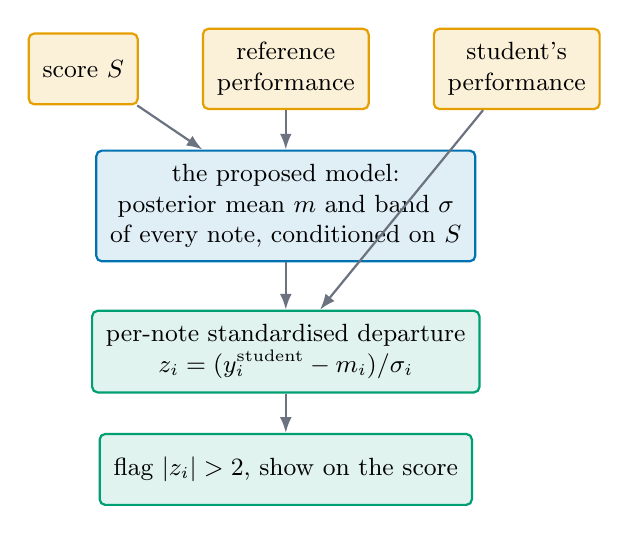
\begin{tikzpicture}[node distance=5mm]
        \node[data] (s) {score $S$};
        \node[data, right=8mm of s] (r) {reference\\performance};
        \node[data, right=8mm of r] (p) {student's\\performance};
        \node[model, below=5mm of r] (m) {the proposed model:\\posterior mean $m$ and band $\sigma$\\of every note, conditioned on $S$};
        \node[res, below=6mm of m] (z) {per-note standardised departure\\$z_i = (y_i^{\text{student}} - m_i)/\sigma_i$};
        \node[res, below=5mm of z] (f) {flag $|z_i| > 2$, show on the score};
        \draw[arr] (s) -- (m); \draw[arr] (r) -- (m); \draw[arr] (p) -- (z);
        \draw[arr] (m) -- (z); \draw[arr] (z) -- (f);
      \end{tikzpicture}}
      \end{center}
    \end{column}
    \begin{column}{0.54\textwidth}
      \small
      \textbf{Reuses} the error-spotting task (AUROC 0.995 on velocity under
      the proposed model), the calibrated bands, and the per-piece
      adaptation. \\[2mm]
      \textbf{Narrative:} the representation is useful because its
      uncertainty makes a judgement actionable: a departure is flagged
      only when it exceeds what the model itself cannot predict. \\[2mm]
      \textbf{What is missing:} no hypothesis is tested. The evaluation
      would be a user study or a teacher's agreement rate, which needs
      participants and ethics approval, neither possible before February.
    \end{column}
  \end{columns}
\end{frame}

\begin{frame}{Option 1: the feedback view (mock, not measured)}
  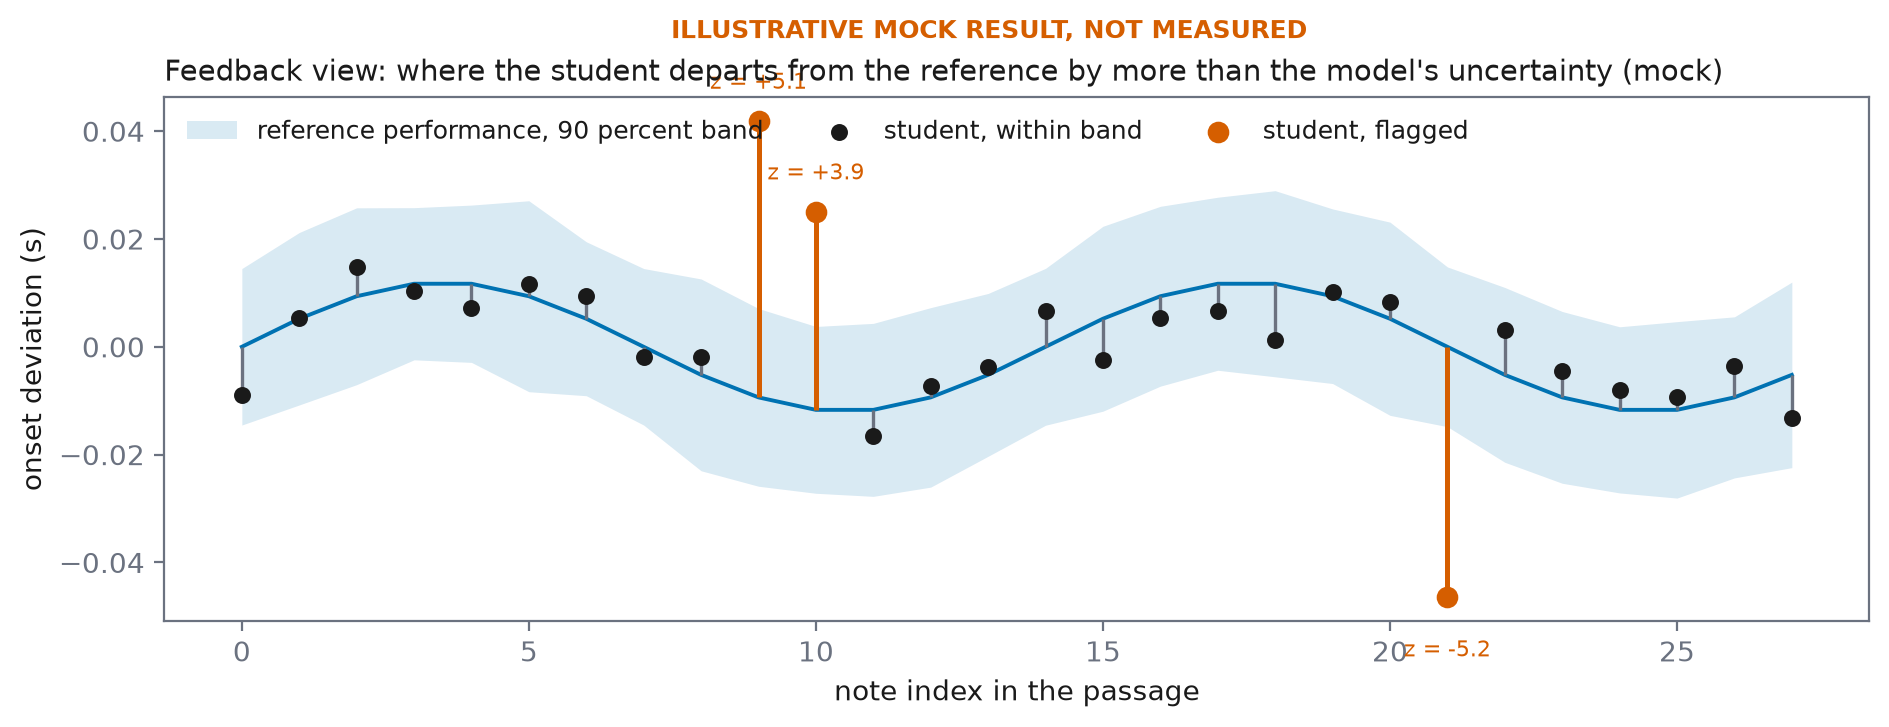
\includegraphics[width=\textwidth]{proposal_feedback_mock.png}
  \vspace{1mm}

  \small Each note of a student's performance is placed against the
  reference performance's posterior, so the band is the model's own
  uncertainty about that note. Three notes fall outside it and are
  flagged. The numbers are hand-set to show the form of the view.
\end{frame}

% ---------------------------------------------------------------------
\begin{frame}{Option 2: the concept, expression follows what the score repeats}
  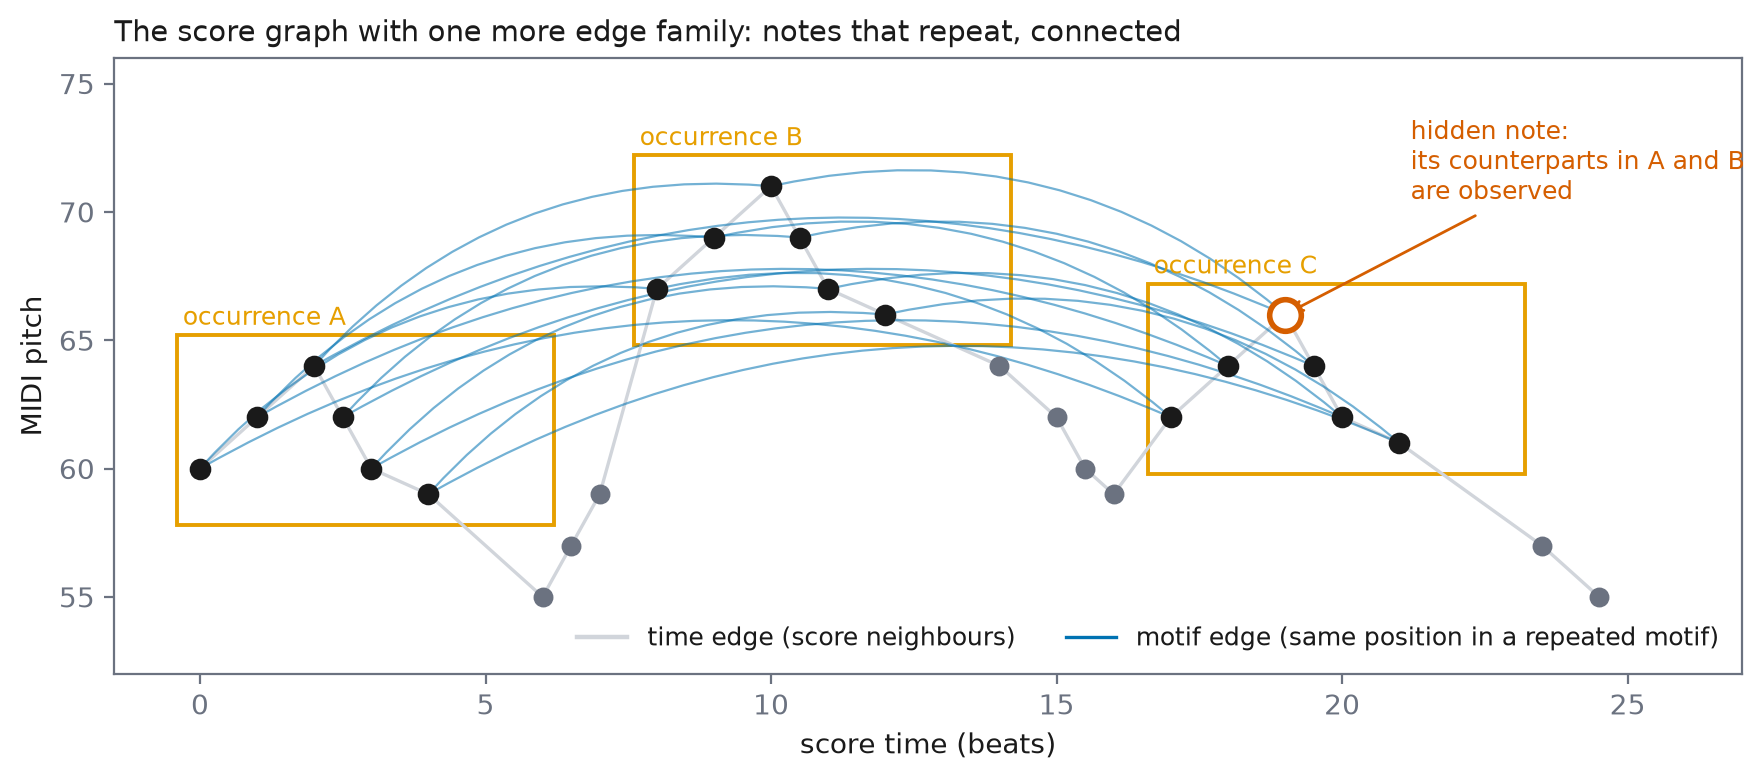
\includegraphics[width=0.86\textwidth]{proposal_motif_graph.png}
  \vspace{1mm}

  \small The current graph connects score neighbours (grey). The motif
  edge family (blue) connects each note of a motif occurrence to the same
  position in the other occurrences, from the BPS-motif annotations or
  from the ISMIR 2026 model's predictions. A hidden note then has two
  kinds of neighbour: the notes around it in time, and the notes that
  \emph{are} it, elsewhere in the piece.
\end{frame}

% ---------------------------------------------------------------------
\begin{frame}{Option 2: methodology, the same model with one more edge family}
  \footnotesize
  \textbf{Model.} The proposed model is unchanged. Only the adjacency gains a term,
  \[
    W = W_{\text{time}} + w_{\text{m}}\, W_{\text{motif}},
  \]
  where $(W_{\text{motif}})_{ij} = 1$ when notes $i$ and $j$ hold the same
  position in two occurrences of one motif, and $0$ otherwise,
  and $K_{\mathcal G} = U\,g(\nu; s)\,U^{\top}$ is built from the Laplacian of $W$
  as before, with $w_{\text{m}}$ learned by the per-piece evidence.
  \vspace{1mm}

  \textbf{Arms}, paired per piece and seed, with the per-piece bias column in every arm:
  time-only graph (the attribution winner), time $+$ pitch (the current
  model), time $+$ annotated motif edges, time $+$ predicted motif edges.
  \vspace{1mm}

  \textbf{Masking.} Hide notes inside motif occurrences whose counterpart
  in at least one other occurrence is observed. Score timing, articulation
  and velocity by paired RMSE and NLL, and coverage of the 90 percent band.
  \vspace{1mm}

  \textbf{Data.} BPS-motif annotates the first movements of all 32
  Beethoven sonatas. ASAP holds 25 of them, over 200 performances, nine
  pieces already inside the thesis's pools. The 400-note excerpts are the
  expositions, where the motif returns.
  \vspace{1mm}

  \textbf{Hypotheses, fixed before the first run.} H1: motif edges improve
  timing and velocity calibration on hidden motif notes against the
  time-only graph. H2: predicted edges retain most of the annotated
  edges' gain. Falsification: an interval that includes zero on H1 means
  the structure performance follows is temporal smoothing, and the thesis
  says so.
\end{frame}

% ---------------------------------------------------------------------
\begin{frame}{Option 2: what the result would look like (mock, not measured)}
  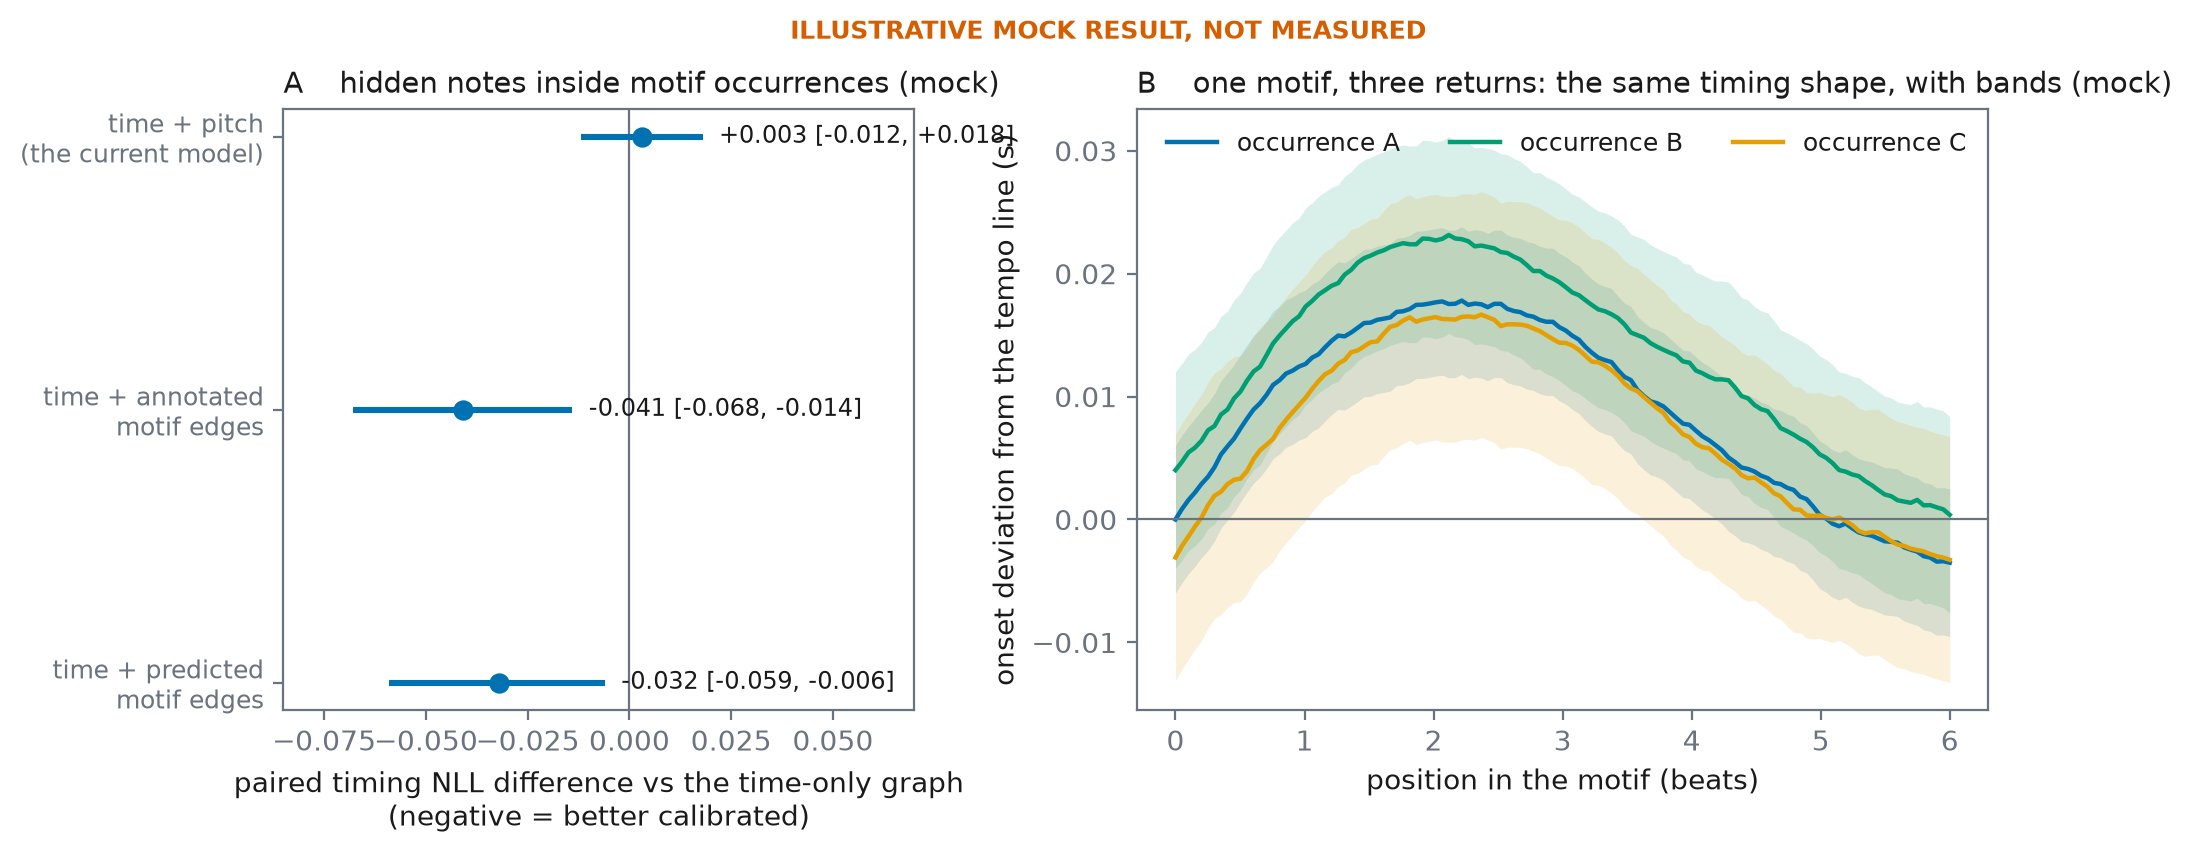
\includegraphics[width=0.95\textwidth]{proposal_mock_results.png}
  \vspace{1mm}

  \small Panel A is the study's one decisive figure: the motif arms
  against the time-only graph on hidden motif notes, with the current
  pitch term shown for scale. Panel B is the application view the same
  posterior gives for free: how one motif was shaped at each of its
  returns, with uncertainty. Both panels are drawn from hand-set numbers
  to show the form of the answer, not its value.
\end{frame}

% ---------------------------------------------------------------------
\begin{frame}{Plan and recommendation}
  \small
  \begin{columns}[T]
    \begin{column}{0.5\textwidth}
      \textbf{Option 2, in five working days}
      \begin{enumerate}
        \item motif edge builder, and ASAP score MIDI aligned to the
          BPS-motif note lists;
        \item hypotheses and masking rule committed before any run;
        \item development runs, four arms, Beethoven pieces, sharded;
        \item write-up: a section in the piano chapter, a slide in the deck;
        \item if H1 holds: one pre-specified evaluation on untouched
          Beethoven performances, before the January talk.
      \end{enumerate}
    \end{column}
    \begin{column}{0.5\textwidth}
      \textbf{What each outcome gives the thesis}
      \begin{itemize}
        \item H1 supported: a direction. Expression follows what the score
          repeats, read motif by motif with uncertainty, and the two
          papers become one line of work.
        \item H1 not supported: the attribution story is complete, tested
          against the most musically plausible alternative.
      \end{itemize}
      \vspace{2mm}
      \textbf{Recommendation.} Option 2. Option 1 can still be built as a
      demo on top of it, since the feedback view only needs the posterior.
      \vspace{2mm}

      \textcolor{muted}{\small The writing freeze of 23 October is reopened
      for this one bounded study.}
    \end{column}
  \end{columns}
\end{frame}

\end{document}
